\documentclass[12pt,a4paper]{article}
\usepackage{amsmath,amssymb,amsthm}
\usepackage{makeidx,graphics}
\usepackage[dvips]{graphicx}
%\usepackage[latin1]{inputenc}
%\usepackage[portuguese]{babel}
\usepackage[utf8]{inputenc}
\usepackage{ae}
\usepackage{indentfirst}
\usepackage{amsbsy}
\usepackage{fancyhdr}
\usepackage{pstricks}
\usepackage[all]{xy}
\usepackage{wrapfig}
\usepackage[pdfstartview=FitH,backref,colorlinks,bookmarksnumbered,bookmarksopen,linktocpage,urlcolor=blue,
linkcolor=cyan]{hyperref}
\usepackage{bussproofs}
\usepackage{amsmath}
\usepackage{mathtools}
\usepackage{amsthm}
\usepackage{amsfonts}
\usepackage{amssymb}
\usepackage{wasysym}
\usepackage{amsbsy}
\usepackage{url}
\usepackage{enumerate}
\usepackage{tikz}
\usepackage{float}
\usepackage{xfrac}
\usepackage{subcaption}
\usepackage{mathrsfs}
\usepackage{pgfplots}
\pgfplotsset{compat=newest}
\usepgfplotslibrary{fillbetween}

\newtheorem{definition}{Definição}
%\newtheorem{example}{Exemplo}
\newtheorem{lema}{Lema}
\newtheorem{teorema}{Teorema}
\newtheorem{corolario}{Corolário}
\newtheorem{obs}{Observação}

\setlength{\topmargin}{-1.0in}
\setlength{\oddsidemargin}{0in}
\setlength{\evensidemargin}{0in}
\setlength{\textheight}{10.5in}
\setlength{\textwidth}{6.5in}
\setlength{\baselineskip}{12mm}

\newcommand{\dx}{\ \mathrm{d} x }
\newcommand{\dy}{\ \mathrm{d} y }
\newcommand{\dz}{\ \mathrm{d} z }
\newcommand{\du}{\ \mathrm{d} u }
\newcommand{\dv}{\ \mathrm{d} v }
\newcommand{\dr}{\ \mathrm{d} r }
\newcommand{\dt}{\ \mathrm{d} t }
\newcommand{\dteta}{\ \mathrm{d} \theta }
\newcommand{\dro}{\ \mathrm{d} \rho }
\newcommand{\dfi}{\ \mathrm{d} \phi }
\newcommand{\ds}{\ \mathrm{d} s }
\newcommand{\dS}{\ \mathrm{d} S }
\newcommand{\dq}{\ \mathrm{d} q }
\newcommand{\dif}{\mathrm{d}}

\DeclareMathOperator{\rot}{rot}
\DeclareMathOperator{\diverg}{div}

\graphicspath{{img/}}

\renewcommand{\sectionmark}[1]{ \markright{ \thesection.\ #1}}

\title{\textbf{Variável Complexa 1}\\ Lista 2}
\author{Caio Tomás de Paula \\ 190011289}
\date{February 14, 2020}

\begin{document}
	\maketitle
\begin{enumerate} 
	\item Sejam $z = a + bi$ e $z_0 = a_0 + b_0i$, com $a,b,a_0,b_0 \in\mathbb{R}$. Temos
	\begin{enumerate}[a)]
		\item  O conjunto $\Re(z)\geq\Re(z_0)$ consiste dos pontos $z$ do plano complexo tais que $a \geq a_0$, i.e., o conjunto 
		\begin{align*}
		A = \left\{ z=a+bi\in\mathbb{C} : a\geq a_0 \text{ com } a,a_0\in\mathbb{R} \right\} \cong \left\{ (x,y)\in\mathbb{R}^2 : x = a_0, a_0\in\mathbb{R} \right\}.
		\end{align*}
		Podemos ver que $A$ consiste de um semiplano do plano complexo:
		\begin{figure*}[h!]
			\centering
			\begin{tikzpicture}[>=latex]	
			\draw[color=white,fill=blue!25] (1,-2)--(1,2)--(3,2)--(3,-2);
			\draw[color=red] (1,-2)--(1,2);
			\draw[->] (-1,0)--(3.5,0) node [at end,right]{$\Re$};
			\draw[->] (0,-2)--(0,2) node [at end,right]{$\Im$};
			\node [at= {(1,0)}, below left ] {$a_0$};
			\end{tikzpicture}
		\end{figure*}
		\par Temos então que $A$ é fechado (pois seu complementar em $\mathbb{C}$ é aberto); sua fronteira é a reta vertical $x=a_0$, em vermelho no desenho; $A$ não é domínio, pois não é aberto; e $A$ é ilimitado.	
	
	\item O conjunto $\Re(z)<\Im(z_0)$ consiste dos pontos $z$ do plano complexo tais que $a < b_0$, i.e., o conjunto 
	\begin{align*}
	B = \left\{ z=a+bi\in\mathbb{C} : a < b_0 \text{ com } a,b_0\in\mathbb{R} \right\} \cong \left\{ (x,y)\in\mathbb{R}^2 : x<b_0, b_0\in\mathbb{R} \right\}.
	\end{align*}
	Podemos ver que $B$ consiste de um semiplano do plano complexo:
	\begin{figure*}[h!]
		\centering
		\begin{tikzpicture}[>=latex]	
		\draw[color=white,fill=blue!25] (-0.5,-2)--(-0.5,2)--(-3,2)--(-3,-2);
		\draw[dashed, color=red] (-0.5,-2)--(-0.5,2);
		\draw[->] (-3.5,0)--(2,0) node [at end,right]{$\Re$};
		\draw[->] (0,-2)--(0,2) node [at end,right]{$\Im$};
		\node [at= {(-0.5,0)}, below right ] {$b_0$};
		\end{tikzpicture}
	\end{figure*}
	\par Temos então que $B$ é aberto (pois seu complementar em $\mathbb{C}$ é fechado); sua fronteira é a reta vertical $x=b_0$, tracejada em vermelho no desenho; $B$ é domínio, pois é aberto e conexo; e é ilimitado.
	
	\item O conjunto $\Re(z^2) \geq 1$ consiste dos pontos $z$ do plano complexo tais que $a^2-b^2 \geq 1$, i.e., o conjunto
	\begin{align*}
	C = \left\{ z = a+bi\in\mathbb{C} : a^2-b^2 \geq 1 \text{ com } a,b\in\mathbb{R}  \right\} \cong \left\{ (x,y)\in\mathbb{R}^2 : x^2-y^2 \geq 1 \right\}.
	\end{align*}
	Podemos ver que $C$ tem então o seguinte esboço:
	\begin{figure*}[h!]
		\centering
		\begin{tikzpicture}
		\begin{axis}[xlabel=$\Re$, ylabel=$\Im$, axis lines=middle, xtick={-1,1}, xticklabels={-1,1}, ytick={}, yticklabels={}, xmax=2.2, xmin=-2.2]
		\addplot[red,samples=200,domain=(1:2),name path=curvadc,thick] {(x^2-1)^(1/2)};
		\addplot[red,samples=200,domain=(1:2),name path=curvadb,thick] {-(x^2-1)^(1/2)};
		\addplot[red,samples=200,domain=(-2:-1),name path=curvaec,thick] {(x^2-1)^(1/2)};
		\addplot[red,samples=200,domain=(-2:-1),name path=curvaeb,thick] {-(x^2-1)^(1/2)};
		\addplot[blue!25] fill between[of=curvaec and curvaeb];
		\addplot[blue!25] fill between[of=curvadc and curvadb];
		\addplot[] coordinates {(-2,0) (-1,0)};
		\addplot[] coordinates {(1,0) (2,0)};
		\end{axis}
		\end{tikzpicture}
	\end{figure*} 
\par Temos, portanto, que $C$ é fechado (pois seu complementar em $\mathbb{C}$ é aberto); sua fronteira é a hipérbole $x^2-y^2=1$ em vermelho; $C$ não é domínio, pois é fechado e não é conexo; e é ilimitado.

\item Seja $D$ o conjunto solução de $\Im(zz_0) > 0$. Temos
\begin{align*}
zz_0 = (a+bi)(a_0+b_0i) = (aa_0 - bb_0) + (b_0a + a_0b)i \Longleftrightarrow \Im(zz_0) = b_0a + a_0b
\end{align*}
e, portanto, 
\begin{align*}
\Im(zz_0) > 0 \Longleftrightarrow b_0a+a_0b > 0.
\end{align*}
Há aqui dois casos:
\begin{enumerate}[(i)]
	\item se $z_0=0$, não há solução, i.e., $D = \emptyset$, que não é nem fechado nem aberto, tem fronteira vazia, não é domínio e é limitado;
	\item se $z_0\neq 0$, então 
	\begin{align*}
	D = \left\{ z = a+bi\in\mathbb{C} : b_0a+a_0b > 0, a,b,a_0,b_0\in\mathbb{R} \right\} \cong \left\{ (x,y)\in\mathbb{R}^2 : b_0x + a_0y > 0 \right\}
	\end{align*}
	que tem o esboço abaixo:
	\begin{figure*}[h!]
		\centering
		\begin{tikzpicture}[>=latex]	
		\draw[color=white,fill=blue!25] (-2,-2)--(-2,2)--(2,2);
		\draw[dashed, color=red,thick] (-2,-2)--(2,2);
		\draw[->] (-2,0)--(2,0) node [at end,right]{$\Re$};
		\draw[->] (0,-2)--(0,2) node [at end,above]{$\Im$};
		%\node [at= {(-0.5,0)}, below right ] {$b_0$};
		\end{tikzpicture}
		\caption*{Aqui consideramos $z_0 = -1+i$, de modo que a reta tracejada é $y=x$.}
	\end{figure*}
	\par Nesse caso, $D$ é aberto, sua fronteira é a reta $b_0x + a_0y = 0$, é domínio e é ilimitado.
\end{enumerate}
\item Seja $E$ o conjunto solução da inequação. Temos 
\begin{align*}
|z - z_0| < |\overline{z} - z_0| &\Longleftrightarrow (a-a_0)^2 + (b-b_0)^2 < (a-a_0)^2 + (-b-b_0)^2 \\ &\Longleftrightarrow 4bb_0 > 0 \\ &\Longleftrightarrow bb_0>0
\end{align*}
Aqui temos dois casos novamente:
\begin{enumerate}[(i)]
	\item se $b_0 = 0$, então $E = \emptyset$, que não é fechado nem aberto, não é domínio, tem fronteira vazia e é limitado;
	\item se $b_0\neq 0$, então temos $b>0$, i.e.,
	\begin{align*}
	E = \left\{ z = a+bi\in\mathbb{C} : b>0, b\in\mathbb{R} \right\} \cong\left\{ (x,y)\in\mathbb{R}^2 : y>0 \right\}
	\end{align*}
	que tem o esboço abaixo:
	\begin{figure*}[h!]
		\centering
		\begin{tikzpicture}[>=latex]	
		\draw[color=white,fill=blue!25] (-3,0)--(-3,3)--(3,3)--(3,0);
		\draw[dashed, color=red,ultra thick] (-3,0)--(3,0);
		\draw[->] (-3,0)--(3,0) node [at end,right]{$\Re$};
		\draw[->] (0,-2)--(0,3) node [at end,above]{$\Im$};
		\end{tikzpicture}
	\end{figure*}
\par Nesse caso, $E$ é aberto, sua fronteira é a reta $x=0$, ele é domínio e é ilimitado.
\end{enumerate}
\item Seja $F$ o conjunto solução da inequação. Temos
\begin{align*}
|z - z_0|\leq |z - \overline{z_0}| \Longleftrightarrow (a - a_0)^2 + (b-b_0)^2 \leq (a-a_0)^2+(b+b_0)^2 \Longleftrightarrow bb_0\geq 0.
\end{align*}
Novamente, temos dois casos:
\begin{enumerate}[(i)]
	\item se $b_0=0$, então $bb_0=0\geq 0, \forall b\in\mathbb{R}$, ou seja, $F = \mathbb{C}$, que é aberto, tem fronteira vazia, é domínio e é ilimitado;
	\item se $b_0\neq 0$, então $bb_0\geq 0 \Leftrightarrow b\geq 0$, de modo que
	\begin{align*}
	F = \left\{ z = a+bi\in\mathbb{C} : b\geq 0, b\in\mathbb{R} \right\} \cong \left\{ (x,y)\in\mathbb{R}^2 : y\geq 0 \right\}
	\end{align*}
	que tem o esboço abaixo:
	\begin{figure*}[h!]
		\centering
		\begin{tikzpicture}[>=latex]	
		\draw[color=white,fill=blue!25] (-3,0)--(-3,3)--(3,3)--(3,0);
		\draw[color=red,ultra thick] (-3,0)--(3,0);
		\draw[->] (-3,0)--(3,0) node [at end,right]{$\Re$};
		\draw[->] (0,-2)--(0,3) node [at end,above]{$\Im$};
		\end{tikzpicture}
	\end{figure*}
\par Nesse caso, $F$ é fechado, sua fronteira é a reta $x=0$, não é domínio e é ilimitado.
\end{enumerate}
\item Seja $G$ o conjunto procurado. Temos 
\begin{align*}
1\leq |z - \overline{z_0}| \leq 3 \Longleftrightarrow 1\leq (a-a_0)^2 + (b+b_0)^2 \leq 9
\end{align*}
Podemos ver, então, que $G$ é uma coroa circular; mais especificamente:
\begin{align*}
G = \overline{D}(\overline{z_0};3)\setminus D(\overline{z_0};1)
\end{align*}
que tem o esboço abaixo:
\begin{figure*}[h!]
	\centering
	\begin{tikzpicture}[>=latex]	
	\draw[color=blue, fill=blue!25](1,1) circle[radius=3];
	\draw[color=blue, fill=white](1,1) circle[radius=1]; 
	\draw[->] (-2,0)--(4,0) node [at end,right]{$\Re$};
	\draw[->] (0,-2)--(0,4) node [at end,above]{$\Im$};
	\node [at= {(1,1)}, above] {$\overline{z_0}$};
	\node [at= {(1,0)}, below] {$a_0$};
	\node [at= {(0,1)}, left] {$-b_0$};
	\draw[dashed] (0,1)--(1,1);
	\draw[dashed] (1,0)--(1,1);
	\node[at={(2,0)}, below] {$a_0+1$};
	\node[at={(4,0)}, below] {$a_0+3$};
	\node[at={(0,2)}, left] {$b_0+1$};
	\node[at={(0,4)}, left] {$b_0+3$};
	\end{tikzpicture}
\end{figure*}
\par Temos que $G$ é fechado, sua fronteira é a união
\begin{align*}
\partial D(\overline{z_0};3)\cup\partial D(\overline{z_0};1),
\end{align*}
ele não é domínio e é limitado.
\item Seja $H$ o conjunto desejado. Temos que
\begin{align*}
\Im(z^2)\leq 1 \Longleftrightarrow 2ab\leq 1 \Longleftrightarrow ab\leq 1/2
\end{align*}
de modo que 
\begin{align*}
H = \left\{ z = a+bi\in\mathbb{C} : ab\leq 1/2, a,b\in\mathbb{R} \right\}\cong\left\{ (x,y)\in\mathbb{R}^2 : xy\leq 1/2 \right\}
\end{align*}
cujo esboço é:
\begin{figure*}[h!]
	\centering
	\begin{tikzpicture}
	\begin{axis}[xlabel=$\Re$, ylabel=$\Im$, axis lines=middle, xtick={-1,1}, xticklabels={-1,1}, ytick={}, yticklabels={}, xmax=3.4, xmin=-3.4, ymax=3.4, ymin=-3.4]
	\addplot[red,samples=500,domain=(-3.3:-0.15),name path=B,thick] {0.5*(1/x)};
	\addplot[red,samples=500,domain=(0.15:3.3),name path=C,thick] {0.5*(1/x)};
	\addplot[blue!25] fill between[of=B and C];
	\addplot[] coordinates {(-3.4,0) (3.4,0)};
	\addplot[] coordinates {(0,-3.4) (0,3.4)};
	\end{axis}
	\end{tikzpicture}
\end{figure*} 
\par Temos que $H$ é fechado, sua fronteira é a hipérbole $\displaystyle{ y = \frac{1}{2x}}$, não é domínio e é ilimitado.
\end{enumerate} 
\item 
\begin{enumerate}[a)]
	\item Temos que 
	$$V = \left\{ z\in\mathbb{C} : |z|\leq 1, \Re(z)\geq\displaystyle{\frac{1}{2}} \right\}$$ 
	é a interseção do disco unitário $\mathbb{D}$ com o semiplano $\Re(z)\geq 1/2$.
	\begin{figure*}[h!]
		\centering
		\begin{tikzpicture}
		\draw[fill=violet!30,thick] (60:2)--(-60:2) arc (-60:60:2);
		\draw[->] (1,1.73)--(1,0.5); 
		\draw[->] (-60:2) arc (-60:30:2) node [at end, right]{$\gamma_2$};
		\draw[-latex] (-1,0)--(3,0) node [at end,right]{$\Re$};
		\draw[-latex] (0,-2)--(0,2) node [at end,above]{$\Im$};
		\node[at={(1,0.5)}, left] {$\gamma_1$};
		\node [at= {(1.4,-0.8)}, above] {$V$};
		\node[at={(1.8,-0.6)}, below right] {$\partial V$};
		\node [at= {(1,0)}, below left] {$\frac{1}{2}$};
		\node [at= {(2,0)}, below right] {$1$};
		\end{tikzpicture}
	\end{figure*}
	Temos, então, que $\partial V = \gamma_1*\gamma_2$, com
	\begin{align*}
	\gamma_1(t) &= \left( \frac{1}{2}; \frac{\sqrt{3}}{2}-\sqrt{3}t \right), t\in[0,1] \\
	\gamma_2(\theta) &= \left( \cos\theta; \sin\theta \right), \theta\in\left[-\frac{\pi}{3},\frac{\pi}{3}\right].
	\end{align*}
	\item Temos que 
	$$ V = \left\{ z\in\mathbb{C} : \frac{1}{2}\leq |z|\leq 1, \Re(z)\geq 0 \right\} $$
	é a interseção da coroa circular
	$$ \mathbb{D}\setminus D(0,1/2) $$
	com o semiplano $\Re(z)\geq 0$:
	\begin{figure*}[h!]
		\centering
		\begin{tikzpicture}
		\draw[fill=violet!30,thick] (-90:2)--(-90:1) arc (-90:90:1) (90:1)--(90:2) arc (90:-90:2);
		\draw[->] (0,2)--(0,1.5) node [at end, left]{$\gamma_1$}; 
		\draw[->] (60:1) arc (60:25:1) node [at end, left]{$\gamma_2$};
		\draw[->] (0,-1)--(0,-1.5) node [at end, left]{$\gamma_3$};
		\draw[->] (-60:2) arc (-60:30:2) node [at end, right]{$\gamma_4$};
		\draw[-latex] (-1,0)--(3,0) node [at end,right]{$\Re$};
		\draw[-latex] (0,-2.5)--(0,2.5) node [at end,above]{$\Im$};
		\node [at= {(0.7,-1.6)}, above] {$V$};
		\node[at={(1.8,-0.6)}, below right] {$\partial V$};
		\node [at= {(0.95,0)}, below left] {$\frac{1}{2}$};
		\node [at= {(2,0)}, below right] {$1$};
		\end{tikzpicture}
	\end{figure*}
\par Temos então $\partial V = \gamma_1*\gamma_2*\gamma_3*\gamma_4$, com
	\begin{align*}
	\gamma_1(t) &= \left(0; 1 -\frac{t}{2} \right), t\in[0,1] \\
	\gamma_2(\theta) &= \frac{1}{2}\left( \cos\theta; -\sin\theta \right), \theta\in\left[-\frac{\pi}{2},\frac{\pi}{2}\right] \\
	\gamma_3(s) &= \left(0; -\frac{1}{2} -\frac{s}{2} \right), s\in[0,1] \\
	\gamma_4(\alpha) &= (\cos\alpha; \sin\alpha), \alpha\in\left[ -\frac{\pi}{2},\frac{\pi}{2} \right].
	\end{align*}
\item Temos que
$$ V = \left\{ z\in\mathbb{C} : \frac{1}{3}\leq |z|\leq 1, \Re(z)\geq\Im(z)\geq 0 \right\} $$
é a interseção dos semiplanos $\Re(z)\geq 0, \Im(z)\geq 0$ (que correspondem ao primeiro quadrante do plano) e $\Re(z)\geq\Im(z)$ (que corresponde à região "abaixo" da reta $x=y$) com a coroa circular
$$ \mathbb{D}\setminus D(0,1/3). $$
Essa região tem a seguinte forma:
	\begin{figure*}[h!]
		\centering
		\begin{tikzpicture}
		\draw[fill=violet!30,thick] (45:3)--(45:1) arc (45:0:1) (0:1)--(0:3) arc (0:45:3);
		\draw[->] (45:1) arc (45:15:1) node [at end, above right]{$\gamma_1$};
		\draw[->] (0:1)--(0:2) node [at end, below]{$\gamma_2$};
		\draw[->] (0:3) arc (0:23:3) node [at end, right]{$\gamma_3$};
		\draw[->] (45:3)--(45:2) node [at end, above]{$\gamma_4$};
		\draw[dashed] (0,0)--(1.41,1.41);
		\draw (0:0.5) arc (0:45:0.5);
		\draw (0:0.5) arc (0:25:0.5) node [at end, above left]{$\frac{\pi}{4}$};
		\draw[-latex] (-1,0)--(4,0) node [at end,right]{$\Re$};
		\draw[-latex] (0,-2)--(0,2) node [at end,above]{$\Im$};
		\node [at= {(2.2,0.7)}] {$V$};
		\node[at={(2.2,2.2)}, right] {$\partial V$};
		\node [at= {(1,0)}, below] {$\frac{1}{3}$};
		\node [at= {(3,0)}, below] {$1$};
		\end{tikzpicture}
	\end{figure*}
\par Temos então $\partial V = \gamma_1*\gamma_2*\gamma_3*\gamma_4$, com
\begin{align*}
\gamma_1(\theta) &= \frac{1}{3}\left( \cos\theta; -\sin\theta \right), \theta\in\left[-\frac{\pi}{4},0\right] \\
\gamma_2(t) &= \left(\frac{1}{3} + \frac{2}{3}t;0 \right), t\in[0,1] \\
\gamma_3(\alpha) &= (\cos\alpha; \sin\alpha), \alpha\in\left[ 0,\frac{\pi}{4} \right] \\
\gamma_4(s) &= \left(\frac{1}{\sqrt{2}} -\frac{2}{3\sqrt{2}}s;\frac{1}{\sqrt{2}} -\frac{2}{3\sqrt{2}}s \right), s\in[0,1] 
\end{align*}
	
	
\end{enumerate}

\end{enumerate}
	
\end{document} 